% ==================================================================
% 3.3 Vibration-Aware Training  <-- DONG GOP CHINH (doi khung 2026-07-26)
%
% LICH SU: ban truoc trinh bay CONSISTENCY la phuong phap chinh. Doi chung
% augment-only (Section 4.2) cho thay augmentation THANG consistency 36.2 vs
% 30.0 retain, nen phuong phap chinh doi thanh augmentation, con consistency
% tro thanh BIEN THE duoc bao cao kem ket qua am. Xem paper/PENDING_ABLATION.md.
% file: sections/07_vibcon.tex
% ==================================================================
\subsection{Vibration-Aware Training}
\label{sec:vibcon}

\begin{figure}[t]
\centering
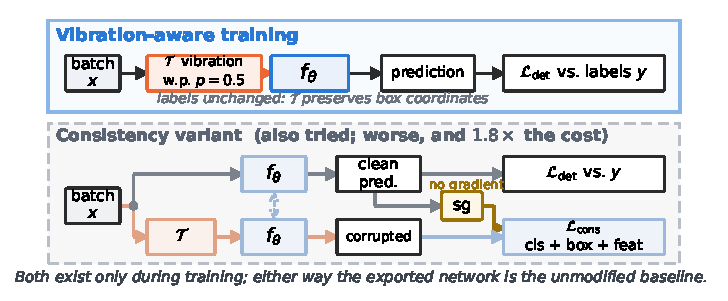
\includegraphics[width=0.95\textwidth]{figures/fig2_method.pdf}
\caption{Vibration-aware training (top) and the consistency variant we also tried
(bottom). The method we recommend is the simple one: corrupt a fraction of each
batch with $\mathcal{T}$ and compute the ordinary detection loss on the corrupted
image. The variant forwards the batch twice and adds a consistency term against a
stop-gradient copy of the clean prediction. Neither survives into deployment: the
exported network is unchanged in either case.}
\label{fig:method}
\end{figure}

Let $\mathcal{T}$ denote the stochastic vibration operator of
Section~\ref{sec:shake}, with severity and blur orientation resampled per batch.
Fig.~\ref{fig:method} contrasts the method with the variant of
Section~\ref{sec:mainresults}; the method is one line. During training, each batch $x$ is replaced by
$\mathcal{T}(x)$ with probability $p = 0.5$, and the ordinary detection loss is
computed on whatever image the network receives:
\begin{equation}
\mathcal{L} = \mathcal{L}_{\det}\bigl(f_\theta(\hat{x}), y\bigr),
\qquad
\hat{x} = \begin{cases}
\mathcal{T}(x) & \text{with probability } p,\\
x & \text{otherwise.}
\end{cases}
\label{eq:vibaware}
\end{equation}
Because $\mathcal{T}$ preserves object coordinates the labels $y$ need no
adjustment, which is what makes the substitution legitimate at all. No module is
added, no second forward pass is required, and the exported graph is structurally
identical to the baseline, so inference cost is unchanged. The only training cost
is the corruption operator, a depthwise convolution and two elementwise
operations.

\subsubsection{Why this is not simply data augmentation as usually understood.}
Standard detection augmentation samples nuisances the training distribution already
contains: flips, scale jitter, colour shifts. $\mathcal{T}$ samples one it does
\emph{not}, because VisDrone is collected from stable platforms. This is therefore
not a regularisation trick but a correction of a mismatch between the data a
detector is trained on and the conditions it will meet, which is why the severities
in Section~\ref{sec:shake} are chosen to bracket rotorcraft flight rather than to
maximise validation score.

\subsubsection{A consistency variant, which we report because it is worse.}
Before running the control, we expected that a stronger signal could be extracted
from the corrupted view than the detection loss provides. The variant forwards both
$x$ and $\mathcal{T}(x)$ through the same weights, computes the detection loss on
the clean branch only, and adds a consistency term that pulls the corrupted
prediction towards a stop-gradient copy of the clean one,
\begin{equation}
\mathcal{L} = \mathcal{L}_{\det}\bigl(f_\theta(x), y\bigr)
 + \lambda_{\mathrm{vib}} \, \mathcal{L}_{\mathrm{cons}}
 \bigl(f_\theta(\tilde{x}),\; \mathrm{sg}[f_\theta(x)]\bigr),
\qquad \lambda_{\mathrm{vib}} = 0.5,
\label{eq:vibcon}
\end{equation}
where $\mathcal{L}_{\mathrm{cons}}$ sums, over pyramid levels, a temperature-scaled
cross-entropy on objectness, a smooth $L_1$ term on boxes gated by clean-branch
objectness, and a squared error between neck features. Exact forms are in the
released code. The stop-gradient is not optional: without it the objective is
minimised by degrading the clean prediction towards the corrupted one, lowering the
loss while destroying the detector. The reasoning was that the clean prediction
says more than the hard label, and that blur destroys exactly that structure.
Section~\ref{sec:mainresults} shows it does not survive measurement.

\subsubsection{Training procedure.}
We apply the corruption as a finetuning stage rather than from scratch: starting
from a converged baseline checkpoint, we finetune for $120$ epochs at batch size
$8$ with gradient accumulation $12$, MuSGD at learning rate $2\times10^{-3}$, and a
three-epoch warm-up before the corruption is switched on. The method can therefore
be applied to a detector that has already been trained, without repeating its
schedule. Checkpoints are selected by clean validation AP, the same rule used for
the baseline, so no checkpoint in this paper is chosen using the robustness
protocol it is evaluated on.
